\chapter{Introduzione}

Nel panorama odierno della sicurezza informatica, ogni secondo conta. Quando un sistema viene compromesso, gli attaccanti lasciano tracce invisibili che esistono solo nella memoria volatile del computer - tracce che svaniscono al riavvio del sistema. È in questo contesto che la Digital Forensics e, in particolare, l'analisi della memoria, assumono un ruolo fondamentale nella risposta agli incidenti e nelle investigazioni digitali.

\section{Contesto e Motivazioni}

\subsection{L'importanza crescente della Digital Forensics nell'era digitale}

Viviamo in un'epoca in cui la trasformazione digitale ha permeato ogni aspetto della società. Dalle infrastrutture critiche ai servizi finanziari, dalla sanità alla difesa nazionale, la dipendenza dai sistemi informatici è totale e irreversibile. Questa digitalizzazione pervasiva ha però un lato oscuro: l'espansione della superficie di attacco e la crescente sofisticazione delle minacce cyber.

Secondo il rapporto Clusit 2025 \cite{clusit2025}, gli attacchi informatici sono aumentati del 27\% a livello globale e del 15\% in Italia rispetto all'anno precedente, con danni economici stimati in miliardi di euro.

\begin{figure}[H]
    \centering
    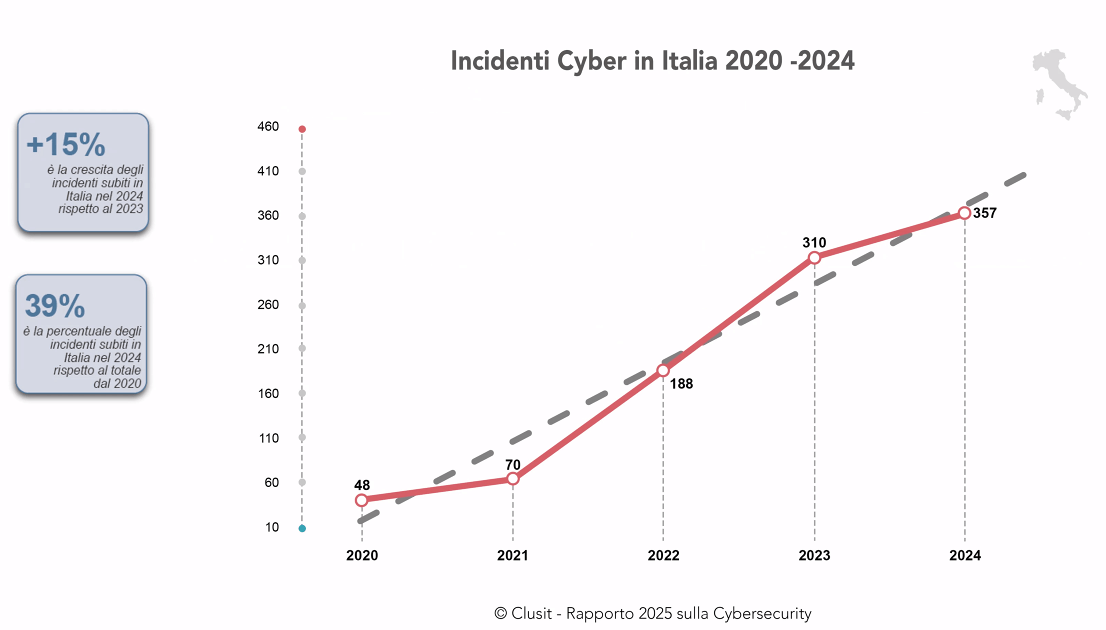
\includegraphics[width=1\linewidth]{images/intro/clusit-ita.png}
\end{figure}

In questo scenario, la Digital Forensics è diventata una competenza essenziale per qualsiasi organizzazione che voglia proteggere i propri asset digitali e rispondere efficacemente agli incidenti di sicurezza. Questa disciplina rappresenta oggi un pilastro fondamentale della cybersecurity aziendale, fornendo le capacità necessarie per rilevare attività malevole che i sistemi di sicurezza tradizionali potrebbero aver mancato, comprendere la portata e l'impatto di un incidente di sicurezza, contenere la minaccia e prevenire ulteriori danni, recuperare i sistemi compromessi e ripristinare le operazioni normali, e infine apprendere dall'incidente per migliorare le difese future.

\subsection{Il ruolo critico dell'analisi della memoria nei processi investigativi}

Tra le varie tecniche di Digital Forensics, l'analisi della memoria RAM occupa una posizione privilegiata. A differenza dell'analisi del disco, che esamina dati persistenti, l'analisi della memoria cattura lo stato "vivo" del sistema al momento dell'acquisizione. Questa capacità unica permette di osservare i processi in esecuzione, compresi quelli nascosti o offuscati dai rootkit che sfuggirebbero a un'analisi tradizionale. Simultaneamente, le connessioni di rete attive rivelano comunicazioni in corso con server di comando e controllo, mentre le chiavi crittografiche, normalmente protette, appaiono in chiaro durante il loro utilizzo. L'analisi della memoria espone inoltre gli artefatti di malware più sofisticati – dal codice iniettato agli hook di sistema, dalle modifiche al kernel alle credenziali temporaneamente decriptate – fornendo una visione completa dell'attività malevola che sarebbe altrimenti invisibile.

L'importanza dell'analisi della memoria è cresciuta esponenzialmente con l'evoluzione delle tecniche di attacco. I moderni malware sono progettati per operare esclusivamente in memoria (fileless malware), lasciando poche o nessuna traccia sul disco. Tecniche come process injection, reflective DLL injection e living-off-the-land rendono l'analisi della memoria non solo utile, ma spesso l'unico modo per rilevare e comprendere un attacco sofisticato.

\subsection{Sfide attuali}

L'analisi della memoria, nonostante la sua importanza critica, continua a incontrare ostacoli significativi che ne limitano la diffusione su larga scala. La complessità tecnica rappresenta la prima barriera: questa disciplina richiede non solo padronanza degli strumenti, ma una comprensione profonda delle strutture interne del sistema operativo, dei meccanismi di gestione della memoria e delle tecniche di anti-forensics adottate dai malware moderni. Tale curva di apprendimento scoraggia molti professionisti che, di fronte alla scelta, preferiscono concentrarsi su domini più consolidati come l'analisi di file system o di log di rete.

A questa complessità intrinseca si somma la sfida del volume dei dati. I sistemi moderni, dotati di decine o centinaia di gigabyte di RAM, producono dump di dimensioni proibitive per un'analisi manuale, richiedendo strumenti automatizzati e tecniche di filtraggio sofisticate per isolare gli artefatti significativi. La natura volatile della memoria aggiunge ulteriore pressione temporale: ogni secondo che passa dopo un incidente aumenta il rischio che evidenze cruciali vengano sovrascritte, trasformando l'acquisizione in una corsa contro il tempo che richiede procedures tanto rapide quanto affidabili.

Dal punto di vista strumentale, l'ecosistema delle soluzioni per la memory forensics rimane frammentato. Il framework open source Volatility rappresenta lo standard di fatto, ma richiede competenze da linea di comando e restituisce output che devono essere interpretati con grande esperienza. Le soluzioni commerciali alternative, pur offrendo interfacce più intuitive, spesso presentano costi elevati e funzionalità che non sempre giustificano l'investimento. La mancanza di automazione nelle operazioni critiche – dall'identificazione dei pattern sospetti alla correlazione tra artefatti, fino alla stesura dei report – trasforma attività che potrebbero essere standardizzate in processi manuali e time-consuming.

L'integrazione dei risultati dell'analisi della memoria con altre fonti di intelligence rappresenta un'ulteriore sfida. La correlazione con log applicativi, traffico di rete o feed di threat intelligence rimane un processo in larga parte artigianale e suscettibile di errori, compromettendo la visibilità complessiva dell'incidente e rallentando la risposta.

È proprio per rispondere a queste sfide che nascono piattaforme come VolWeb \cite{volweb2024}, concepite per democratizzare l'accesso alla memory forensics attraverso interfacce intuitive, automazioni intelligenti e capacità di correlazione avanzate, riducendo drasticamente la barriera d'ingresso e aumentando l'efficacia delle investigazioni.

\section{Obiettivi della Tesi}

Questo lavoro di tesi si propone di affrontare le sfide identificate attraverso l'espansione e il miglioramento di VolWeb, una piattaforma web-based per l'analisi forense della memoria. L'obiettivo principale consiste nell'integrazione di un sistema completo per la gestione e l'applicazione di regole YARA, strumento fondamentale per l'identificazione di pattern e malware nei dump di memoria. 

Questa integrazione, dettagliata nel Capitolo 5, mira a trasformare VolWeb in una piattaforma capace di gestire centralmente le regole YARA, applicarle efficacemente durante le analisi forensi e presentare i risultati in modo che faciliti l'interpretazione da parte degli analisti. Il sistema proposto permette non solo l'upload e la validazione delle regole, ma anche la loro organizzazione in rulesets logici, facilitando l'applicazione sistematica di intere categorie di pattern durante le investigazioni.

Il secondo obiettivo riguarda la validazione della piattaforma in contesti operativi reali, presentata nel Capitolo 6, con particolare riferimento alla preparazione per l'esercitazione NATO CCDCOE Locked Shields 2026. Questa validazione include stress test della piattaforma in condizioni di carico elevato, con analisi concorrenti di dump multipli, situazione tipica durante incident response su larga scala dove molteplici endpoint devono essere analizzati simultaneamente. La sperimentazione sul campo fornisce inoltre metriche concrete sull'efficacia delle espansioni implementate e feedback operativo per future ottimizzazioni.

Questi obiettivi non sono meramente tecnici, ma rispondono a un'esigenza concreta del mondo della cybersecurity: rendere l'analisi della memoria accessibile, efficiente e integrata nel workflow di incident response moderno. I capitoli che seguono tracciano il percorso completo dalla teoria alla pratica: il Capitolo 2 fornisce le basi teoriche del DFIR e della memory forensics, il Capitolo 3 analizza VolWeb nella sua versione originale, il Capitolo 4 presenta l'esperienza di Locked Shields che ha motivato le espansioni, il Capitolo 5 dettaglia l'implementazione delle nuove funzionalità, il Capitolo 6 ne valida l'efficacia sul campo, e infine le conclusioni sintetizzano i risultati raggiunti e delineano le prospettive future.